\documentclass[11pt]{beamer}
\usetheme{Warsaw}
\usepackage[utf8]{inputenc}
\usepackage[portuguese]{babel}
\usepackage[T1]{fontenc}
\usepackage{amsmath}
\usepackage{amsfonts}
\usepackage{amssymb}
\usepackage{graphicx}
\author{Leandro, Diego e Alexandre}
\title{k-Nearest Neighbors algorithm (KNN)}
%\setbeamercovered{transparent} 
%\setbeamertemplate{navigation symbols}{} 
%\logo{} 
%\institute{} 
%\date{} 
%\subject{} 
\begin{document}

\begin{frame}
\titlepage
\end{frame}

\begin{frame}
\tableofcontents
\end{frame}

\section{Introdução}
% ALEXANDRE
\begin{frame}{Objetivo}
	\begin{itemize}
	\item Realizar um estudo sobre a aplicação do algoritmo KNN em FPGAs;
	\item Reconhecimento de indivíduos a partir dos movimentos e dados
	antropométricos;
	\item Foi realizado uma conexão entre o Kinect, a placa Altera Cyclone
	(2C35) e o computador para coleta em tempo real dos dados;
	\item Construindo um ambiente experimental simulado. 
	\end{itemize}
\end{frame}

% DIEGO
\begin{frame}{Kinect Versão 2}

\begin{itemize}
	\item O Kinect é equipado com uma câmera RGB-D sensível à profundidade.
	\item O processador de imagens do SDK do Kinect usa as imagens RGB-D para
	calcular as posições das articulações da pessoa.
\end{itemize}

\end{frame}

\begin{frame}{Kinect Versão 2}

\begin{itemize}
	\item Cada articulação do mapa de profundidade representa um ponto em uma
	caixa 3D, naquela coordenada (x, y, z) em particular;
	\item Se o valor da articulação é (0, 0, 0), isso indica essa articulação
	está no ponto central dessa caixa 3D.
\end{itemize}

\end{frame}

% LEANDRO
\begin{frame}{Algoritmo KNN}

\begin{itemize}
	\item O algoritmo K-NN é utilizado para classificar um objeto não rotulado,
	baseado no rótulo de seus vizinhos mais próximos;
	\item Essa proximidade é baseada em uma métrica de distância entre dois
	pontos (distância Euclidiana);
	\item A regra de classificação do k-NN é associar a uma amostra de teste, o
	rótulo da maioria das categorias de seus “k” vizinhos mais próximos;
\end{itemize}

\end{frame}


\section{Processo de implementação do algoritmo KNN em VHDL}
% ALEXANDRE
\begin{frame}{Descrição do bloco operativo}
	\begin{itemize}
	\item O bloco operativo é dividido basicamente em 3 loops;
	\item Os pontos recebidos pela parte de aquisição de dados vem no padrão
	IEEE 754;
	\item Megafunctions:
		\begin{itemize}
		\item Memória
		\item Subtrator
		\item Somador
		\item Multiplicador
		\item SQRT
		\item Comparador de ponto flutuante
		\end{itemize}
	\end{itemize}
\end{frame}

\begin{frame}{Descrição do bloco operativo}
	\begin{itemize}
	\item Memória
	\begin{figure}[ht]
	\centering
	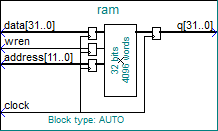
\includegraphics[width=.5\textwidth]{ram}
	\label{fig:ram}
	\end{figure}
	\end{itemize}
\end{frame}

\begin{frame}{Descrição do bloco operativo}
	\begin{itemize}
	\item Somador - Subtrator
	\begin{figure}[ht]
	\centering
	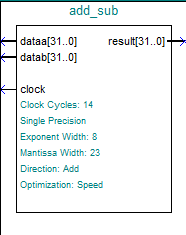
\includegraphics[width=.5\textwidth]{add_sub}
	\label{fig:add_sub}
	\end{figure}
	\end{itemize}
\end{frame}

\begin{frame}{Descrição do bloco operativo}
	\begin{itemize}
	\item Multiplicador
	\begin{figure}[ht]
	\centering
	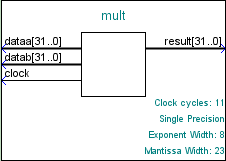
\includegraphics[width=.5\textwidth]{mult}
	\label{fig:mult}
	\end{figure}
	\end{itemize}
\end{frame}

\begin{frame}{Descrição do bloco operativo}
	\begin{itemize}
	\item Raiz quadrada
	\begin{figure}[ht]
	\centering
	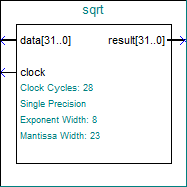
\includegraphics[width=.5\textwidth]{sqrt}
	\label{fig:sqrt}
	\end{figure}
	\end{itemize}
\end{frame}

\begin{frame}{Descrição do bloco operativo}
	\begin{itemize}
	\item Compara se dataa é menor que datab
	\begin{figure}[ht]
	\centering
	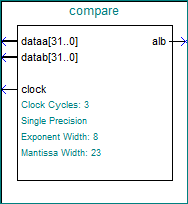
\includegraphics[width=.5\textwidth]{compare}
	\label{fig:compare}
	\end{figure}
	\end{itemize}
\end{frame}

\begin{frame}{Descrição do bloco operativo}
	\begin{figure}[ht]
	\centering
	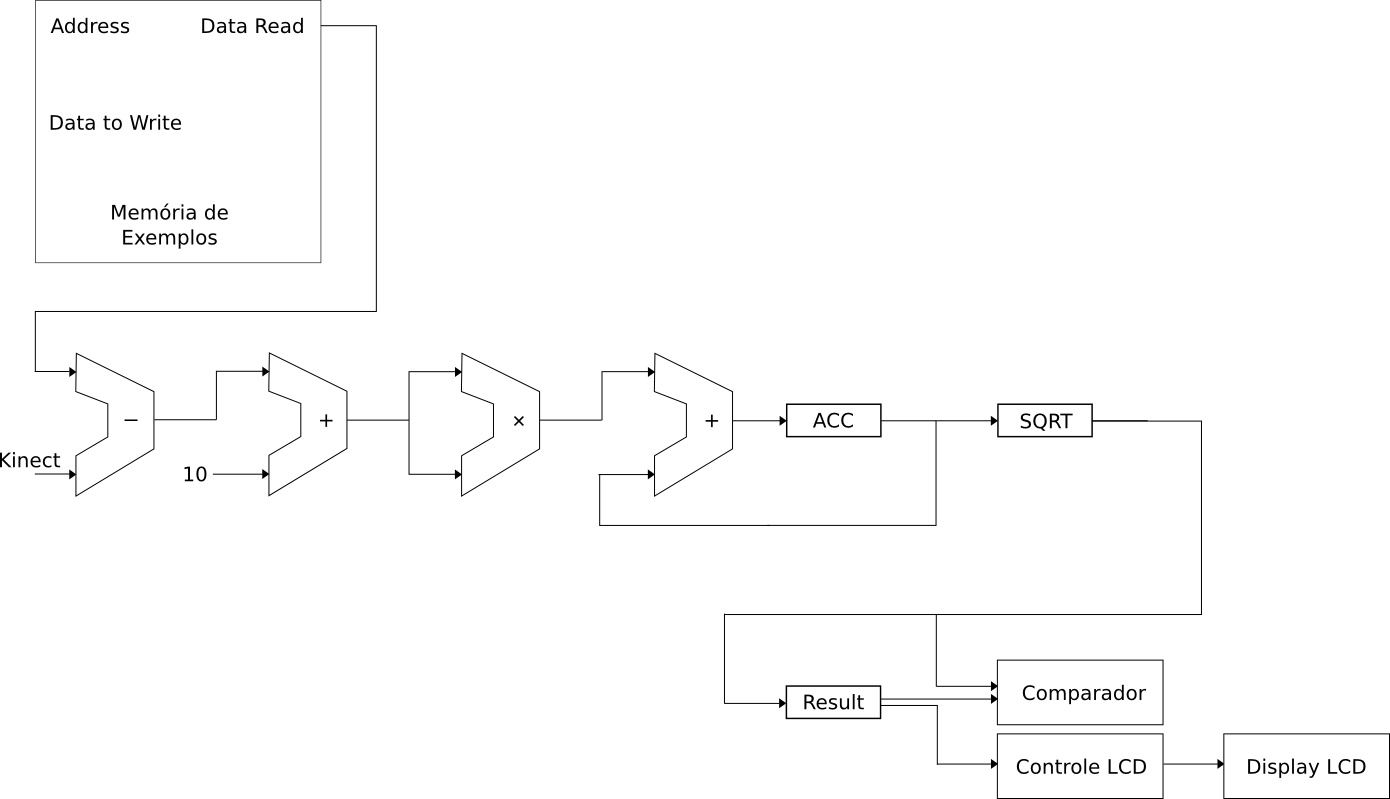
\includegraphics[width=1.0\textwidth]{knn_sem_controle}
	\label{fig:knn_sem_controle}
	\end{figure}
\end{frame}

% LEANDRO SÓ COPIA O TRECHO DE CÓDIGO ABAIXO PARA CIRAR UM NOVO SLIDE
\begin{frame}{Descrição do bloco de controle}
	\begin{figure}[ht]
	\centering
	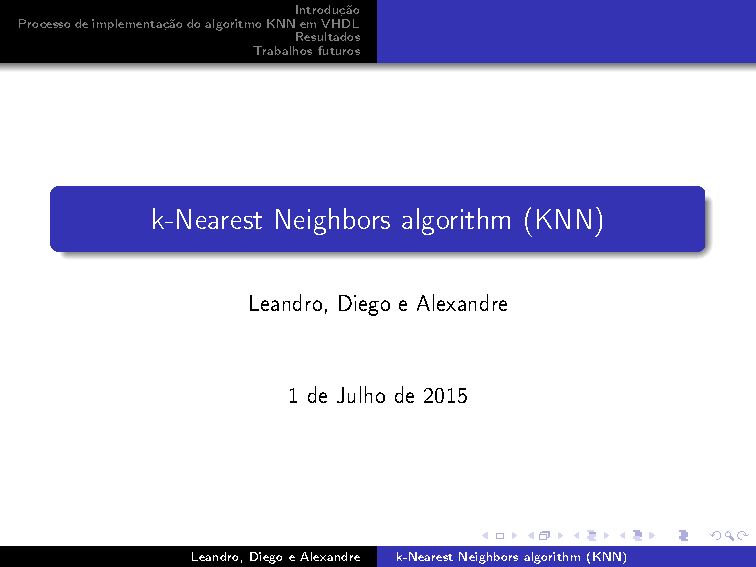
\includegraphics[width=1.0\textwidth]{knn}
	\label{fig:knncalc}
	\end{figure}
\end{frame}

\begin{frame}{Descrição do bloco de controle}
	\begin{figure}[ht]
	\centering
	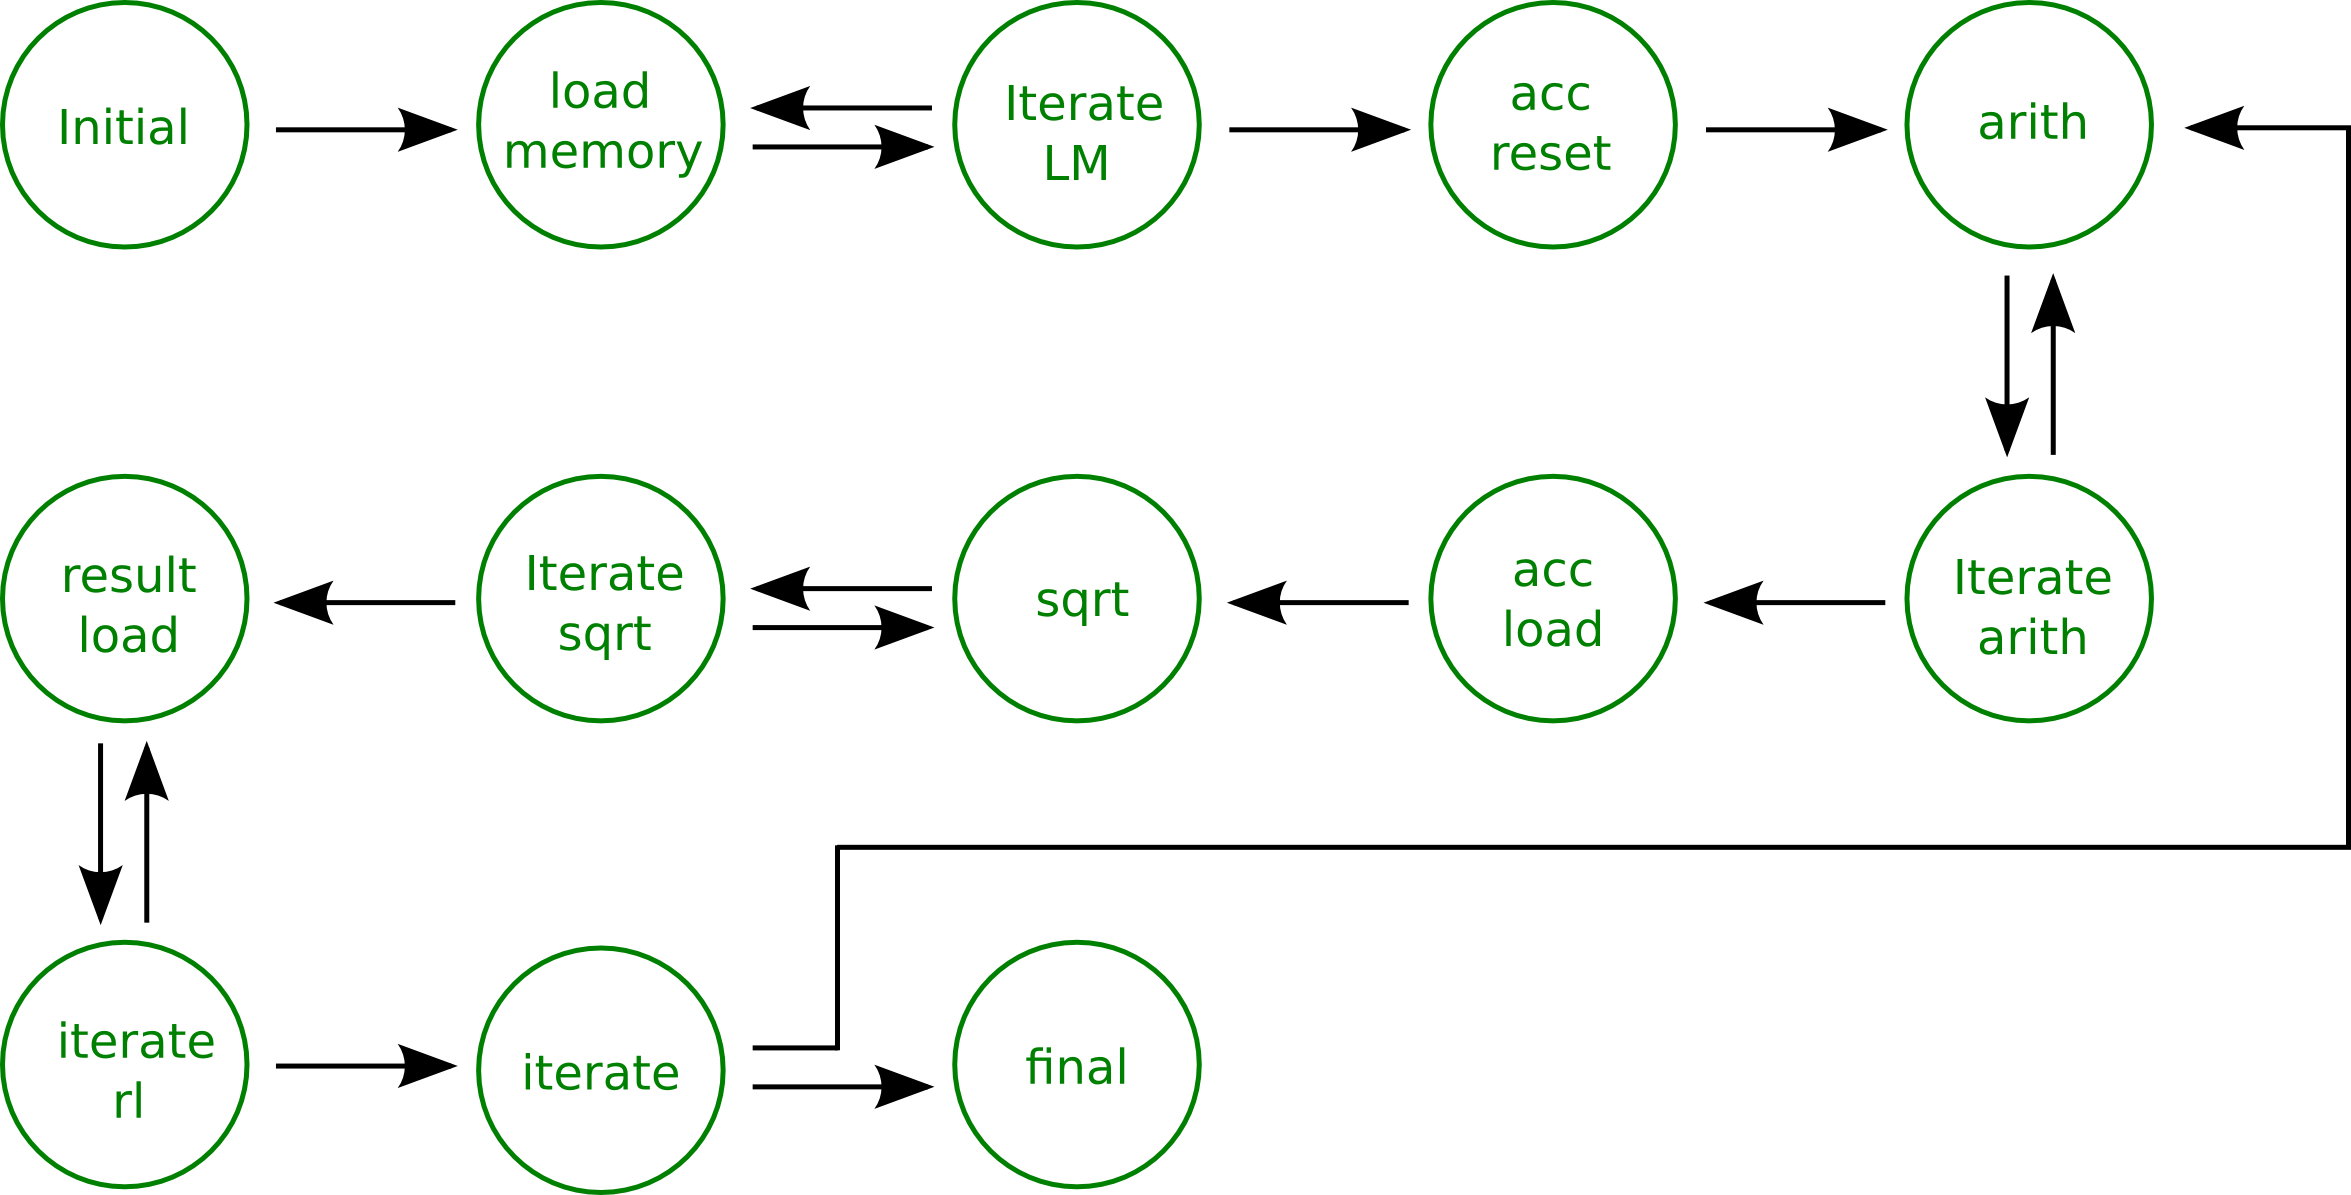
\includegraphics[width=1.0\textwidth]{control_unit}
	\label{fig:control_unit}
	\end{figure}
\end{frame}

% FIM DA IMPLEMENTAÇÃO DO CALCULO DO KNN

\section{Resultados}
% DIEGO
\begin{frame}{Resultados}

\begin{itemize}
	\item O algoritmo M5Rules atingiu 99\% de acerto, gerou a árvore no
	Weka e rodou na placa;
	\item O KNN chegou a 99\% de acerto na placa.
\end{itemize}

\end{frame}

\end{document}